\documentclass{article}
\usepackage[utf8x]{inputenc}
\usepackage{mathtools}
\usepackage{amsmath}
\usepackage{amssymb}
\usepackage{graphicx}
\usepackage{tikz}
\usepackage{pgfplots}
\pgfplotsset{compat=1.15}
\usepackage{mathrsfs}
\usetikzlibrary{arrows}
\usepackage[version=4]{mhchem}
\usepackage{chemfig}
\numberwithin{equation}{section}
\numberwithin{figure}{section}

\title{\textbf{Important Formulae in Physics, Chemistry and Math for JEE}}
\author{S. Sheersh}
\date{21 April 2022}
\newcommand{\Cr}{\times}
\DeclareMathOperator{\adj}{adj}
\newcommand{\Det}[1]{|#1|}
\newcommand{\Sub}[1]{\textsubscript{#1}}
\newcommand{\Sup}[1]{\textsuperscript{#1}}
\begin{document}
\maketitle
\section{Physics}
\begin{enumerate}

	\item Energy of a Wave(for a length $dx$ at $x$): 
		\begin{align}
			dU &=\frac{1}{2}T\left(\frac{\partial y}{\partial x} \right)^2dx\\
			=dK &=\frac{1}{2} \mu v^2 \left(\frac{\partial y}{\partial x} \right)^2dx=\frac{1}{2}\mu v^2_{y} dx
		\end{align}

	\item Energy for a Wavelength worth of length: 
\begin{equation}
 \int_{0}^{\lambda}2\cdot\frac{1}{2}\mu \omega^2\|\psi\|^2 dx
\end{equation}
\begin{equation}
\equiv  \int_{0}^{\lambda}2\cdot\frac{1}{2}\mu \omega^2\| A(\sin(kx-\omega t))\|^2 dx\bigg |_{t=0} 
\end{equation}
\begin{equation}
	\mu \omega^2 A^2 \int_{0}^{\lambda}(\sin^2(kx))dx=\boxed{\mu \omega^2 A^2 \frac{\lambda}{2}} 
\end{equation}
\item Poisson's ratio:
\begin{equation}
	\nu=-\frac{d \epsilon_{\text{trans}}}{d\epsilon_{\text{axial}}}	
\end{equation}
	\item Young Laplace Equation:
		For any general surface there exist two radii of curvature $R_1$ and $R_2$. The Young Laplace equation relates the pressure difference across the surface solely due to surface tension:
\begin{equation}
	\Delta p= \sigma \left(\frac{1}{R_1}+\frac{1}{R_2}\right)
\end{equation}
	\item Some Fundamental Values:
		\begin{enumerate}
			\item $hc=1240 \ eV \ nm $
			\item $2.303 \frac{RT}{F}=0.06$
		\end{enumerate}
	\item Dipoles:
		\begin{enumerate}
			\item Potential due to electric dipole:
				\begin{equation}\Psi(r)=\frac{1}{4\pi\epsilon_0}\frac{\vec{p}\cdot\vec{r} }{r^3}\end{equation}
			\item Field due to electric dipole:
				\begin{equation}
					E_{r}=\frac{1}{4\pi\epsilon_0}\frac{2p\cos(\theta)}{r^3}
				\end{equation}
				\begin{equation}
					E_{\theta}=\frac{1}{4\pi\epsilon_0}\frac{p\sin(\theta)}{r^3}
				\end{equation}
			\item Field due to magnetic dipole:
				\begin{equation}
					\mathbf{B(r)}=\frac{\mu_0}{4\pi}\left(\frac{3\mathbf{r(m\cdot r)}}{r^5}-\frac{\mathbf{m}}{r^3}\right)
				\end{equation}
			\item Field due to magnetic dipole of radius $a$ on its axis:
				\begin{equation}
					B(z)=\frac{\mu_0 I a^2}{2 (a^2+z^2)^{\frac{3}{2}}}
				\end{equation}
		\end{enumerate}
	\item Moseley's Law:
		\begin{equation}
			\sqrt{\nu}=a(Z-b)
		\end{equation}
	\item For a radially symmetric medium, the modification $r \mu \sin(\theta)$ is used instead of $\mu \sin(\theta)$. (It just works, idk why)
	\item Relation between $Q$ and $E_{th}$:
		\begin{equation}
			E_{th}=\left(1+\frac{m}{M}\right) Q
		\end{equation}
		where $m$ is the mass of incoming particle while $M$ is the mass of the particle at rest. (*Can be generalised by using $\frac{M+m}{M}$ and then interpreting some kind of total mass)
	\item When moving up the plane, the slope of surface of the liquid in container is:
		\begin{equation}
			\tan(\theta)=\frac{a+g \sin(\alpha)}{g\cos(\alpha)}
		\end{equation}
	\item Magnetic field due to a moving charge $q$ :
		\begin{equation}
			\vec{B}=\frac{\mu_0}{4\pi}\frac{q(\vec{v}\Cr\vec{r})}{r^3}
		\end{equation}
	\item In a perfectly elastic collision, the two particles exchange their vector momenta.
	\item Displacement current:
		\begin{equation}
			i_d=\epsilon_0 \frac{d\Phi_E}{dt}
		\end{equation}
	\item In free expansion of any gas(including non-ideal ones), $\Delta U$ is conserved. Thus only for an ideal gas is $\Delta T$ also equal to $0$.
	\item For diffraction, minima at: $$\theta=\frac{n\lambda}{a}$$
		where $n\neq 0$, $\lambda$ is the wavelength and $a$ is the width of the slit
	\item Angle of deflection for scattering:
		\begin{equation}
			\phi=\tan^{-1}\left(\frac{|k|}{bv^2}\right)
		\end{equation}
		where $b$ is the distance of closest approach, $v$ is the initial/final velocity(at $r\rightarrow \infty$), and the potential(potential per mass if you want to be picky) is of the form $V(r)=\frac{k}{r}$
	\item Impedance in an AC circuit is calculated as in a DC circuit (i.e $$Z_1+Z_2$$ for series and $$Z_1\oplus Z_2=\left(\frac{1}{Z_1}+\frac{1}{Z_2}\right)^{-1}$$ for parallel), using the fact that impedance for inductor is $$Z_L=i\omega L$$ and for capacitor is $$Z_C=\frac{1}{i\omega C}=-i\frac{1}{\omega C}$$
	\item For an ideal gas, the Kinetic Energy per unit volume is: $$T_{V}=\frac{\rho C_v T}{M}$$, and thus when applying Bernoulli's principle on the motion of an ideal gas use this in the $T_i$ part inside the container 
	\item Facts about a standing wave:
		\begin{itemize}
			\item Near the anti-node potential energy of the particles, when they reach their extreme position, is minimum
			\item Any two particles vibrates either in same phase or out of phase.
			\item Near the anti-node kinetic energy of the particles, when they crosses their mean position, is maximum.
			\item Any two particles having minimum separation $\frac{\lambda}{2}$  may vibrate with same amplitude.
		\end{itemize}
	\item For calculating flux, consider a SPHERE OR A CUBE as a bounding Gaussian surface.
	\item For calculating acceleration when the magnitude of the velocity is constant, use:
		\begin{equation}
			a=v\frac{d\theta}{dt}
		\end{equation}
	\item Force between two plates of the capacitor:
		\begin{equation}
			F=\frac{q^2}{2A\epsilon_0}=\frac{\sigma^2 A}{2\epsilon_0}
		\end{equation}
	\item Power of a lens is $\frac{1}{f_{lens}}$ where $f_{lens}>0$ for convex lens and $f_{lens}<0$ for concave lens.
	\item Power of a \textbf{mirror} is $-\frac{1}{f_{mirror}}$ where $f_{mirror}>0$ for \textbf{convex mirror} and $f_{mirror}<0$ for \textbf{concave mirror}.
	\item If in confusion, try to find the wavelength of the sound signal first(which is independent of the velocity of the observer) and then reason out that if you even have to take the observer velocity in account when using the Doppler finally in the end.
	\item Height of water level in a capillary:
		\begin{align}
			h&=\frac{2T}{R_m \rho g}\\
			&=\frac{2T\cos(\theta)}{r \rho g}\label{suf}
		\end{align}
		where $R_m$ is the radius of the meniscus, $r$ is the radius of the tube  and \ref{suf} occurs when the tube is of sufficient length.\\
		\textbf{Corollary:} When tube is of the sufficient length, $R_m=\dfrac{r}{\cos(\theta)}$ 
	\item If the piston moves without acceleration, the pressure across both sides is constant and thus the process is isobaric
	\item If in a YDSE question, the medium between the slits and the screen also has $\mu_{m}>1$, and the glass inserted is of index $\mu$, use $$\left(\dfrac{\mu}{\mu_m}-1\right)t$$ to calculate the path difference
	\item If a question asks about moving a charge/mass away from the centre of a symmetric distribution, they are asking you to move it along an axis that preserves the symmetry.
	\item Intensity of an electromagnetic wave:
		\begin{equation}
			I=(\text{Energy Density})(\text{Speed of the radiation})=\left(\frac{1}{2}\epsilon_0 E^2\right)(c)
		\end{equation}
	\item Range of communication:
		\begin{equation}
			D=\sqrt{2R h_{t}}+\sqrt{2R h_{r}}
		\end{equation}
		where $h_t$ is the height of the transmitter and $h_r$ the height of the receiver.
	\item For a body of liquid with height $h$, it is very useful to take the average pressure as $(\rho gh/2)$ and multiply it over the surface area in contact to get the force.
	\item Centre of masses and Moment of inertia of different objects:
		\begin{enumerate}
			\item Ring: C=(0,0),I =$MR^2$
			\item
		\end{enumerate}
	\item Current due to a stream of electrons:
		\begin{equation}
			i=ne A v_{d}	
		\end{equation}
	\item End correction in a resonance tube:
		\begin{enumerate}
			\item For a tube open at one end: $$e=0.6 r=0.3 D$$
			\item For a tube open at both ends: $$e=1.2 r=0.6 D$$
		\end{enumerate}
	\item End correction in potentiometer:
		\begin{equation}
		e=\left | \frac{(R_1\ell_2)-(R_2\ell_1)}{R_1-R_2}\right |
		\end{equation}
	\item Loss in kinetic energy due to collision:
		\begin{equation}
			\frac{1}{2}\mu v_{\text{rel}}^2
		\end{equation}
	\item Potential inside a uniformly charged non-conducting sphere at a distance x from the centre :
		\begin{equation}
			V=\frac{1}{4\pi \epsilon_0} \frac{Q}{2R}(3-\frac{x^2}{R^2})
		\end{equation}
		where Q is the total charge on the sphere, R is the radius of the sphere and $x<R$ 
	\item $d$ due to Fresnel biprism in YDSE:
		\begin{equation}
			d=2a(\mu-1)\alpha
		\end{equation}
	\item Orbits:
		\begin{enumerate}
			\item Semi-major axis:
				\begin{equation}
					a=\frac{r_{min}+r_{max}}{2}
				\end{equation}
			\item Eccentricity:
				\begin{equation}
					e=\frac{R-r}{R+r}
				\end{equation}
			\item The angular momentum is preserved (Kepler's second law), and thus $r_1 v_1= r_2 v_2$ for any $r_1 \text{ and } r_2$ on the orbit.
		\end{enumerate}
\end{enumerate}
\section{Chemistry}
\begin{enumerate}
	\item Entropy Formulae
\begin{equation}
	\Delta S_{sys}=n C_v \ln\left(\frac{T_2}{T_1}\right)+n R \ln\left(\frac{V_2}{V_1}\right)
\end{equation}
\begin{equation}
	\Delta S_{sys}= n C_p \ln\left(\frac{T_2}{T_1}\right)- n R \ln\left(\frac{p_2}{p_1}\right)
\end{equation}
	\item Gibbs Free Energy
\begin{equation}
	dG=Vdp-SdT
\end{equation}
	\item Applications of definition of enthalpy:
		\begin{equation}
			\Delta H=\Delta U+\Delta(PV)=\Delta U+\Delta n_g RT
		\end{equation}
		(Even applies to phase change reactions)
	\item Degree of Unsaturation:
\begin{equation}
	DU=(n_{C}-1)-\left(\frac{n_{H}+n_{X}-n_{N}}{2}\right)
\end{equation}
	\item Interplanar crystal spacing of cubic crystal families $(h \ k \ l)$ is defined as
		\begin{equation}
		d_{hkl} = \frac{a}{\sqrt{h^2+k^2+l^2}}.
		\end{equation}
	\item Height of the HCP unit cell: $$ h_{hcp}=4\sqrt{\frac{2}{3}}r$$
	\item Base area of the HCP unit cell: $$A_{hcp}=6\sqrt{3}r^2$$
	\item Electrode Reactions:
		\begin{enumerate}
			\item Electrode reaction of reduction of Oxygen:
		\begin{equation}
			O_{2(g)}\ + 4H^{+}\ + 4 e^{-} \rightarrow 2H_2 O
		\end{equation}
			\item Calomel electrode:
				\begin{equation}
					{\displaystyle {\ce {{Cl^{-}}(4M)|{Hg2Cl2(s)}|{Hg(l)}|Pt}}}
				\end{equation}
				\begin{equation}
					\text{Anode: }	{\displaystyle {\ce {Hg2^2+ + 2e^- <=> 2Hg(l)}},\qquad {\ce {with}}\quad E_{{\ce {Hg2^2+/Hg}}}^{0}=+0.80\ {\ce {V}}}
				\end{equation}
				\begin{equation}
				- \text{ Cathode: }	{\displaystyle {\ce {Hg2Cl2 + 2e^- <=> 2Hg(l) + 2Cl^-}},\qquad {\ce {with}}\quad E_{{\ce {Hg2Cl2/Hg, Cl-}}}^{0}=+0.27\ {\ce {V}}}
				\end{equation}
		\end{enumerate}
	\item Formulae for conductivity:
		\begin{enumerate}
			\item \begin{align}
					R &=\rho\frac{l}{A}\\
					G &=\frac{1}{R} = \frac{1}{\rho}\frac{A}{l}=\kappa \frac{A}{l}\\
					G*=\frac{l}{A} &=R\Cr\kappa\\			
					\Lambda_{m} &=\frac{\kappa}{C}(\text{Unit: S cm\textsuperscript{2} mol\textsuperscript{-1}})\\
					\text{For unit l and A: } G &= \frac{\kappa A}{l}=\kappa\\
					\Rightarrow \Lambda_{m}&=\kappa\\
					\text{For molar volume:  } \Lambda_{m}=\kappa\Cr V	
			\end{align}
		\end{enumerate}
G* is calculated using an electrolyte with known conductivity
	\item Anode is the terminal where oxidation occurs and where the \emph{conventional current enters the circuit};\textbf{ in a battery or a source of DC, it is the \emph{negative terminal }} \emph{but} \textbf{in a passive load(e.g. an electrolytic cell), it is the \emph{positive terminal.}}
	\item The meaning of Van Der Waal's constants:
		\begin{itemize}
			\item \emph{a}: It is the proportionality constant, and the $\left(\dfrac{n}{V}\right)^2$ comes from the fact that pressure depends on both force of repulsion and the frequency of collisions both of which are reduced by factors of concentration ($=\dfrac{n}{V}$)
			\item \emph{b}	$$ b=4N_{A} V_{molecule} $$
		\end{itemize}
	\item \begin{table}[h!]
		\begin{tabular}{|l|l|}
			\hline
			System       & Symmetries                               \\ \hline
			Triclinic    & None                                     \\ \hline
			Monoclinic   & One $C_2$ axis                             \\ \hline
			Orthorhombic & 3 $\perp C_2$ axes                         \\ \hline
			Rhombohedral & One $C_3$ axis                             \\ \hline
			Tetragonal   & One $C_4$ axis                             \\ \hline
			Hexagonal    & One $C_6$ axis                             \\ \hline
			Cubic        & Four $C_3$ axes in tetrahedral arrangement \\ \hline
		\end{tabular}
		\end{table}
	\item Closest distance between octahedral and tetrahedral void in fcc lattice: $$d_{oct\ to\ tet}=\sqrt{\frac{3}{2}}r=\frac{\sqrt{3}}{4}a$$
	\item The configuration for $[Cu(NH_3)_4]^{2+}$ is (showing copper electrons) $3d^8 4p_{z}^1$ while the electrons from $(NH_3)$(or any other SFL), go into the $d_{x^2-y^2},s, p_{x}$ and $p_{y}$ orbitals 
	\item pH of a solution of salt of weak acid+strong base(all logs in base 10):
		\begin{equation}
			pH=\frac{pK_{w}+pK_{a}+\log(C)}{2}=7+\frac{1}{2}pK_{a}+\frac{1}{2}\log(C)
		\end{equation}
	\item pH of a solution of salt of weak base+strong acid(all logs in base 10):
		\begin{equation}
			pH=\frac{pK_{w}-pK_{b}-\log(C)}{2}=7-\frac{1}{2}pK_{b}-\frac{1}{2}\log (C)
		\end{equation}
	\item pH of a solution of salt of weak base+weak acid(all logs in base 10):
		\begin{equation}
			pH=\frac{pK_{w}+pK_{a}-pK_{b}}{2}=7+\frac{1}{2}pK_{a}-\frac{1}{2} pK_{b}
		\end{equation}
	\item $\beta$-D glucopyranose is more stable than $\alpha$-D glucopyranose.	
	\item The chemical potential of the substance is equal to its Gibbs free Energy:
		\begin{equation}\label{cp}
		\mu^{\circ}(A)=\Delta G^{\circ}_{A}
		\end{equation}
	\item For a liquid-gas equilibrium:
		\begin{equation}\label{lg}
			\mu^{\circ}_{A}(g)=\mu^{\circ}_{A}(l)+RT\ln(\chi_{A})
		\end{equation}
		$\chi_{A}$ is the mol fraction of A in the mixture (liquid phase)
	\item For a solid-liquid equilibrium:
		\begin{equation}
			\mu^{\circ}_{A}(l)=\mu^{\circ}_{A}(s)+RT\ln(\chi_{A})
		\end{equation}
		where $\chi_{A}$ is same as above
	\item To find the ebullioscopic constant rewrite \ref{lg} as:
		\begin{align}\label{s1}
			\ln(\chi_A)=\frac{\mu^{\circ}_{A}(g)-\mu^{\circ}_{A}(l)}{RT}\\
			=\frac{\Delta_{vap}G^{\circ}}{RT}
		\end{align}
	Differentiate \ref{s1}by temperature to get
		\begin{align}
			\frac{d\ln(\chi_A)}{dT}=\frac{\partial\frac{\Delta G}{RT}}{\partial T}=-\frac{\Delta H}{RT^2}\\
			\Rightarrow d\ln(\chi_A)=-\frac{\Delta H}{RT^2}dT
		\end{align}
	because $$ \frac{\Delta G}{T}=\frac{\Delta H}{T}-\Delta S.$$\\
	Integrate this back using the limits $T_b$ to $T_b+\Delta T$, to get:
		\begin{equation}
			\ln(\chi_A)=\frac{\Delta H}{R}\left(\frac{1}{T_b}-\frac{1}{T_b+\Delta T}\right)
			\approx \frac{\Delta H}{RT^2}\Delta T
		\end{equation}
	Now, in a binary solution $\chi_A=1-\chi_B$. Assuming $\chi_B <<1$($\because$ Dilute condition)
		\begin{equation}
			\ln(1-\chi_B)=-\chi_B=-\frac{\Delta H}{RT^2}\Delta T
		\end{equation}
		 which means:
		 \begin{equation}
			 \boxed{K_b=1/\frac{\Delta H}{RT^2}=\frac{RT^2}{\Delta H}}
		 \end{equation}
	\item Non-metals generally melt at a higher temperature than metals of the same group.
	\item $[Co(NH_3)_4Cl_2]Cl$ is a diamagnetic compound.
	\item Efficiency of an electrolytic cell:
		\begin{equation}
			\eta=\frac{\Delta G^{\circ}}{\Delta H^{\circ}}=1-T\frac{\Delta S^{\circ}}{\Delta H^{\circ}}
		\end{equation}
	\item In the 3d series, when the lower elements (Sc, Ti, V) get oxidised, they almost always lose all of their $4s$ and $3d$ electrons and acquire the $[Ar]$ noble gas configuration. Thus their oxides (like VO\Sub{2}\Sup{+})are less oxidising than, say Cr\Sub{2}O\Sub{7}\Sup{2-} or MnO\Sub{4}\Sup{-}
	\item Di-carboxylic acids($HOOC-(CH_2)_{n}-COOH$) on heating give different products:
		\begin{enumerate}
			\item For $n=0$(Oxalic acid): Forms $HCOOH$ and $CO_2$
			\item For $n=1$(Malonic acid): Forms $CH_3-COOH$ and $CO_2$
			\item For $n=2,3$(Succinic, Glutaric acid): Forms the respective 5-membered and 6-membered ring anhydride
			\item For $n\geq 4$(Adipic onwards): They start forming cyclic ketones
		\end{enumerate}
	\item The Gold Number is the minimum weight (in milligrams) of a protective colloid required to prevent the coagulation of 10 ml of a standard hydro gold sol when 1 ml of a 10\% sodium chloride solution is added to it
	\item $H_2 O_2$ oxidises $[Fe (CN)_6]^{4-}$ to $[Fe(CN)_6]^{3-}$ in acidic medium but reduces $[Fe(CN)_6]^{3-}$ to $[Fe(CN)_6]^{4-}$ in alkaline medium.
	\item In determining reactivity with H\Sub{2}/Pt or any other reagent with surface playing a dominant role, the least hindered compound will most easily adsorb and thus will react faster with such reagents
	\item H\Sub{3}PO\Sub{4} is used for elimination of alcohols.
	\item Gases(ideal and real):
		\begin{enumerate}
			\item Boyle's Temperature:
				\begin{equation}
					T_{bo}=\frac{a}{Rb}
				\end{equation}
			\item Critical Temperature:
				\begin{equation}
					T_{c}=\frac{8a}{27 Rb}
				\end{equation}
			\item Critical Pressure:
				\begin{equation}
					P_{c}=\frac{a}{27b^2}
				\end{equation}
			\item Critical Volume:
				\begin{equation}
					V_{c}=3b
				\end{equation}
		\end{enumerate}
	\item $ P_{\text {final }}=\sqrt{P_{x}^{o} \times P_{y}^{o}}$ for a very special case of minimum composition of one of the substances to have minimum mole fraction in vapour phase
	\item As branching increases among isomeric alkanes, stability increases and hence heat of combustion decreases

	\item If molality and molarity of any species in a solution is numerically the same, it is same for all the components and for it,numerical value of ml of solution = numerical value of gm of solvent
	\item Rate of diffusion of a gas from an orifice:
		\begin{equation}
			r_{\text{eff}}=\frac{P A}{\sqrt{2\pi M_{gas}RT}}N_{A}
		\end{equation}
		where $P$ is the pressure of the container, $A$ is the area of the orifice, $M_{gas}$ is the molar mass of the gas. 
	\item Coagulating value= (millimoles of electrolyte used)/(volume of sol coagulated in L)  
	\item $\mathrm{R-CONH2\ + HNO_2\rightarrow R-COOH+N_2}$
	\item Lyophillic sols are highly viscous
	\item Reactions of $\mathrm{MnO_{4}^{-}}$:
		\begin{enumerate}
			\item In acidic medium: $\mathrm{MnO_{4}^{-} \rightarrow Mn^{2+}}$
			\item In neutral medium: $\mathrm{MnO_{4}^{-} \rightarrow MnO_2}$
			\item In basic medium: $\mathrm{MnO_{4}^{-} \rightarrow MnO_4^{2-}}$

		\end{enumerate}
	\item Disiamylborane($\mathrm{Sia_2BH}$) is an organoborane used in organic synthesis. It is used for hydroboration–oxidation reactions of terminal alkynes, giving aldehydes via anti-Markovnikov hydration followed by tautomerization
	\item O\Sub{3} is diamagnetic.
	\item Coagulation value is the millimoles of an electrolyte that must be added to 1 L of a colloidal solution for complete coagulation. 
	\item Beckmann rearrangement is the conversion of oxime to amide.
	\item DCC converts -OH into a good Leaving Group
	\item DIBAL-H is an electrophilic reducing reagent.
	\item $1 \mathrm{Debye}= \frac{1}{c}\times 10^{-21} \mathrm{C-m}\approx 3.335 \times 10^{-30}\mathrm{C-m}$
	\item Reactions of $K_2 Cr_2 O_7$:
		\begin{enumerate}
			\item In acidic medium: 
		\end{enumerate}
	\item Alum: $\mathrm{KAl(SO_4)_2}.12H_2 O$
	\item Allenes with different groups on the two terminal carbons are optically active if there are an even number of double bonds in the allene, while those with odd number of double bonds are not.
\end{enumerate}
\section{Math}
\begin{enumerate}
	\item Triangle Inequalities:
\begin{equation}
	|z_1+z_2|\leq|z_1|+|z_2|
\end{equation}
\begin{equation}
	|z_1-z_2|\geq ||z_1|-|z_2||
\end{equation}
	\item BAC-CAB rule:
\begin{equation}
	\vec{a}\Cr(\vec{b}\Cr\vec{c})=\vec{b}(\vec{a}\cdot\vec{c})-\vec{c}(\vec{a}\cdot\vec{b})
\end{equation}
	\item Wallis' Formula:
\begin{equation}
	\int_{0}^{\frac{\pi}{2}} \sin^{n}(x)\cdot \cos^{m}(x)dx=\frac{[(n-1)(n-3)(n-5)\dots 2\ or \ 1][(m-1)(m-3)(m-5)\dots 2 \ or \ 1 ]}{(m+n-0)(m+n-2)(m+n-4)\dots 2 \ or \ 1} K
\end{equation}
\begin{equation}
	\text{where }    K= 
	\begin{dcases}
		\frac{\pi}{2} ,& \text{if }  m \text{ and } n \text{ are even}\\
		        1,              & \text{otherwise}
	\end{dcases}
\end{equation}			
	\item Box product tricks:
		\begin{enumerate}
			\item \begin{equation}\left[(\vec{a}\Cr \vec{b}) \  (\vec{b}\Cr \vec{c}) \ (\vec{c}\Cr\vec{a})\right]=\left[\vec{a} \vec{b} \vec{c}\right]^2\end{equation}
			\item 
				\begin{equation}
					\left[\vec{a} \vec{b} \vec{c}\right]^2=
					\begin{vmatrix}
						\vec{a}\cdot\vec{a} & \vec{a}\cdot \vec{b} & \vec{a}\cdot\vec{c}\\
						\vec{b}\cdot\vec{a} & \vec{b}\cdot\vec{b} & \vec{b}\cdot\vec{c}\\
						\vec{c}\cdot\vec{a} & \vec{c}\cdot\vec{b} & \vec{c}\cdot\vec{c}
					\end{vmatrix}
				\end{equation}
			\item \begin{equation}
					(\vec{a} \Cr \vec{b}) \cdot (\vec{c} \Cr \vec{d})=(\vec{c} \cdot \vec{a})(\vec{d}\cdot\vec{b})-(\vec{c}\cdot\vec{b})(\vec{d}\cdot\vec{a})
				\end{equation}
		\end{enumerate}
	\item Complex Numbers:
		\begin{enumerate}
			\item Expansion of $|1-\alpha_r|$ and $|1-\alpha_r|$ where $\alpha_r$ is the r\textsuperscript{th} root of unity:
				\begin{equation}
					|1-\alpha_r|=\left|1-\cos\left(\frac{2\pi r}{n}\right)-i\sin\left(\frac{2\pi r}{n}\right)\right|=2\left| \sin\left(\frac{\pi r}{n}\right)\right|
				\end{equation}
			*Use half angle formula and then that $|cis(x)|$ has mod 1
		\end{enumerate}
	\item Triangle Centers:
		\begin{enumerate}
			\item The centroid $G$ lies on the line joining Orthocentre $H$ and Circumcentre $O$:
				\begin{centering}
					\begin{figure}[h]
						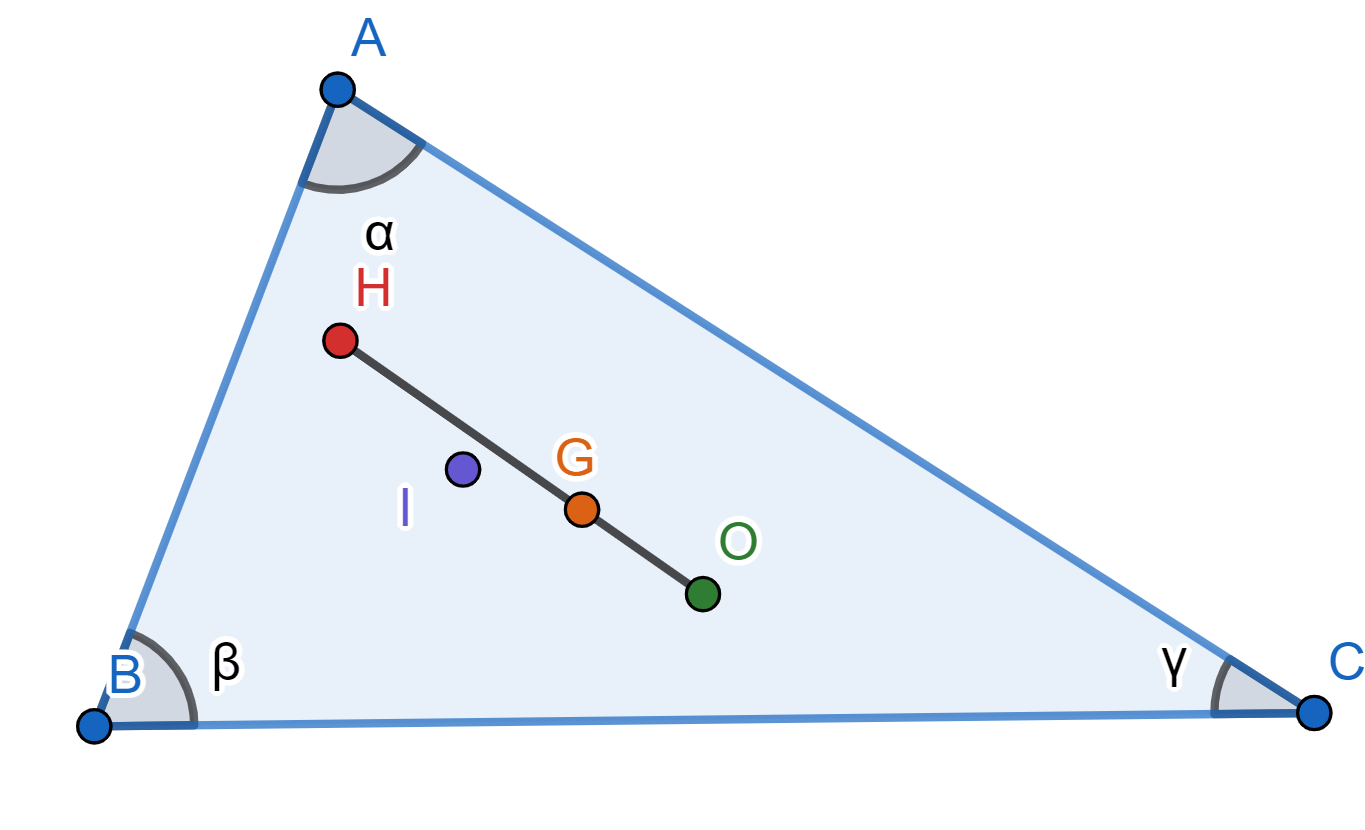
\includegraphics[scale=0.25]{Triangle_Pic.png}
					\end{figure}
				\end{centering}
			\item Orthocentre $H$: \begin{equation}H= \left(\vec{a}+\vec{b}+\vec{c}\right)\end{equation}
			\item The distance of orthocentre $H$ from vertex $A$ is:
				\begin{equation}
					HA= 2R\cos(A)
				\end{equation}
			The distance of orthocentre $H$ from side $a(=BC)$ is (where $D$ is the foot of $\perp$ from $A$):
				\begin{equation}
					HD=2R\cos(B)\cos(C)
				\end{equation}
		\end{enumerate}
	\item For angles $A,B, C$ of a triangle:
		\begin{equation}
			\cos^2(A)+\cos^2(B)+\cos^2(C)=1-2\cos(A)\cos(B)\cos(C)
		\end{equation}
	\item Taylor series of $\tan(x)$:\begin{equation} \tan(x)\approx x+\frac{1}{3}x^3+\frac{2}{15}x^5+\dots\end{equation}
		\item \begin{equation} \text{The coefficient of } x^r \text{ in } (1-x)^{-n} \text{ is } {{n+r-1} \choose {r}} \end{equation} 
		\item But for choosing, you use $${{n+r-1} \choose {r-1}} $$ 
		\item Lagrange Interpolation:
			For a set of $k+1$ data points $(x_0,y_0)\dots (x_k,y_k)$ where no two $x_i, x_j$ are the same, there exists a \emph{Interpolation Polynomial of Lagrange Form}:
			\begin{equation}
				L(x):=\sum_{j=0}^{k} y_j \ell_j(x)
			\end{equation}
			where each $\ell_i$ is the Lagrange basis:
			\begin{equation}
				\ell _{j}(x):=\prod _{\begin{smallmatrix}0\leq m\leq k\\m\neq j\end{smallmatrix}}{\frac {x-x_{m}}{x_{j}-x_{m}}}={\frac {(x-x_{0})}{(x_{j}-x_{0})}}\cdots {\frac {(x-x_{j-1})}{(x_{j}-x_{j-1})}}{\frac {(x-x_{j+1})}{(x_{j}-x_{j+1})}}\cdots {\frac {(x-x_{k})}{(x_{j}-x_{k})}}
			\end{equation}
		\item   \begin{itemize}
			\item	Blank plane is one region 
			\item	Every line adds a region to the plane 
			\item	Every point of intersection adds one more region
			\end{itemize}
		\item   If $A$ is a skew-symmetric matrix of odd dimension, its determinant is always $0$ 
		\item If stuck in a problem where Lagrange Mean Value theorem looks likely, take the function $g(x)=f(x)-x$ and then try the properties on it.
		\item For a system of $3\Cr3$ linear equations:
			\begin{itemize}
				\item Unique solution if $\Delta\neq 0$
				\item No solution if $\Delta = 0$ but at least one of $\Delta_1$, $\Delta_2$ and $\Delta_3$ is non zero
				\item Infinite solutions if $\Delta=\Delta_1=\Delta_2=\Delta_3=0$
			\end{itemize}
		\item Sophie-Germain's Identity:
			\begin{equation}
				a^{4} + 4b^{4} = (a^{2}+2b^{2}-2ab)(a^{2}+2b^{2}+2ab)
			\end{equation}
		\item $BB^{T}$ is a symmetric matrix
		\item if $P(z_1)$ and $Q(z_2)$ are two points on the circle $|z|=r$, the complex number representing the intersection of tangents is $$\frac{2 z_1 z_2}{z_1+z_2}$$
		\item To count the number of rectangles in a regular polygon, find the number of diagonals passing through the centre
		\item If there is a regular n-gon on a unit circle the product of lengths $$(A_1 A_2)(A_1 A_3)(A_1 A_4)\dots (A_1 A_n)=n$$
		\item In the previous point, remember that if $n$ is even then there exists a body diagonal too. 
		\item For an ellipse at the origin, a tangent with slope $m$ is:
			\begin{equation}
				y=mx \pm \sqrt{a^2 m^2 + b^2}
			\end{equation}

			And for a hyperbola it is:
			\begin{equation}
				y=mx \pm \sqrt{a^2 m^2 - b^2}
			\end{equation}
		\item REMEMBER: If asked for non consecutive in combinatorics question, think "gaps"
		\item Think rotation of planes, think of angles between the normals of the plane
		\item Anytime you encounter an integral which involves something like $\dfrac{x^2-1}{x^2+1}$ try putting in $t=x+\frac{1}{x}$. for eg.:
			\begin{align*}
				I &=\int_{1}^{\sqrt{2}+1}\frac{x^2-1}{x^2+1}\frac{1}{\sqrt{1+x^4}}dx
			\\        &=\int_{1}^{\sqrt{2}+1}\frac{(1-\frac{1}{x^2})dx}{(x+\frac{1}{x})\sqrt{x^2+\frac{1}{x^2}}}
			\end{align*}
		\item Stewart's theorem is a powerful theorem for Solutions of Triangles, and can be easily used to derive much stronger results than the hard to remember m-n rule. The theorem:
			\begin{align}
				\text{If in a } \Delta \text{ABC, a point } D \text{ divides } BC \text{ in } m \text{ and } n,\ then\\
				\boxed{b^2 m +c^2 n=a(l^2+mn)}
			\end{align}
		\item The foot of the perpendicular from any focus of the ellipse to any tangent to the ellipse must lie on the auxiliary circle of the ellipse 
		\item The foot of perpendicular from the focus on any tangent to the parabola must lie on the tangent at the vertex to the parabola which in a way can be thought as the auxiliary circle of the parabola

		\item If there is a differential equation like \begin{equation}\label{saneeq}\frac{dy}{dx}+P(x)y=0,\end{equation} it is linear i.e. for solutions $y_1 \text{ and } y_2$, $\lambda y_1+\mu y_2$ is also a solution for $\lambda ,\mu \in \mathbb{R} $. However if there is a non homogeneous part and the equation now becomes \begin{equation}\label{insaneeq}\frac{dy}{dx}+P(x)y=Q(x),\end{equation}and $y_1$ and $y_2$ are again some solutions, $\lambda y_1+\mu y_2$ is not a solution for general $\lambda$ and $\mu$(Check by putting $y_1$ and $y_2$ and into the Diff Eq \ref{insaneeq}  then  checking $\lambda y_1 +\mu y_2$ doesn't satisfy \ref{insaneeq} unless $\lambda+\mu=1$)

		\item If some integral with trig functions isn't working, try substitution by $\tan(\frac{x}{2})$

		\item If there is a problem asking for min/max anywhere, and things look hopeless, try Cauchy-Schwarz inequality:
			\begin{equation}
				|\left<\bf{u},\bf{v}\right>|^2\leq \left<\bf{u},\bf{u}\right>.\left<\bf{v},\bf{v}\right>
			\end{equation}
		where $\left<\cdot, \cdot \right>$ is the inner product and $\bf{u}$ and $\bf{v}$ are vectors, which basically means list of numbers of any kind
		\item For summation of $\sum_{r=1}^n 2^r \tan(2^{r}\theta)$, remember:
			\begin{align}
				\tan(\theta)=\cot(\theta)-2\cot(2\theta)\\
				\tan(2\theta)=\cot(2\theta)-4\cot(4\theta)\\
				\vdots\\
				\tan(2^n\theta)=\cot(2^n\theta)-2^{n+1}\cot(2^{n+1}\theta)
			\end{align}
		\item Adjoint properties:
			\begin{enumerate}
				\item $\adj(A)=\Det{A}A^{-1}$,$\Rightarrow \Det{\adj(A)}=\Det{A}^{n-1}$
				\item $\adj(\adj(A))=\Det{A}^{n-2} A$
			\end{enumerate}
		\item Number of surjective/onto functions $f:A\rightarrow B$ with $\Det{A}=m$ and $\Det{B}=n$($m>n$) is:
			\begin{equation}
				n^m-{n \choose 1}{(n-1)^m}+{n \choose 2}{(n-2)^m}-{n \choose 3}{(n-3)^m}+\dots+(-1)^r{n \choose r}+\dots
			\end{equation}
			using the principle of inclusion and exclusion
		\item Equation of tangent to parabola:
			\begin{equation}
				ty=x+at^2
			\end{equation}
			or 
			\begin{equation}
				y=mx+\frac{a}{m}
			\end{equation}
		\item The product of the perpendiculars on the tangent from the foci is equal to $b^2$.
		\item The reflection of point A on the angle bisectors BE and CF lies on the side BC
		\item SOT Formulas:
		\begin{enumerate}
			\item Length of the median AD of a triangle:
				\begin{equation}
					l_{a}=\frac{1}{2}\sqrt{2b^2+2c^2-a^2}
				\end{equation}
			\item Length of the internal angle bisector of triangle from A:
				\begin{equation}
					d^2_{a}=\frac{bc}{(b+c)^2}\left((b+c)^2-a^2\right)
				\end{equation}
		\end{enumerate}
		\item For a chord of a conic section S=0, with its mid point at (h,k), the formula is:
			\begin{equation}
				T=S_1
			\end{equation}
		\item $(P\Rightarrow Q)\Leftrightarrow(\neg P \vee Q)$
		\item \begin{equation}
				  \neg (\forall x) P(x) \Leftrightarrow (\exists x)(\neg P(x));
			\end{equation}
			  \begin{equation}
				    \neg (\exists x) P(x) \Leftrightarrow (\forall x)(\neg P(x)).
			  \end{equation}
		\item For a system of quadratic equations which has one common root $\alpha$
			\begin{align}
				a_1 x^2 + b_1 x + c_1 &=0\\
				a_2 x^2 + b_2 x + c_2 &=0
			\end{align}
			We can put in $\alpha^2$ and $\alpha$ respectively to form
			\begin{align}
				a_1 \alpha^2 + b_1 \alpha + c_1 &=0\\
				a_2 \alpha^2 + b_2 \alpha + c_2 &=0
			\end{align}
			and then using the cross product formula, we write:
			\begin{align}
				\frac{\alpha^2}{b_1 c_2-b_2 c_1}=\frac{\alpha}{c_1 a_2-c_2 a_1}=\frac{1}{a_1 b_2 - a_2 b_1}
			\end{align}
			and thus equate the values of $\alpha$ from the equations to get:
			\begin{equation}
				\alpha=\frac{(b_1 c_2 - b_2 c_1)}{(c_1 a_2 - c_2 a_1)}=\frac{(c_1 a_2 - c_2 a_1)}{(a_1 b_2 - a_2 b_1)}
			\end{equation}
			\begin{equation}
				\Rightarrow (b_1 c_2 - b_2 c_1)(a_1 b_2 - a_2 b_1)=(c_1 a_2 - c_2 a_1 )^2
			\end{equation}
			\begin{equation}
				\Rightarrow \boxed{\Delta_{bc} \Delta_{ab}=\Delta^2_{ca}}
			\end{equation}
		\item If thinking about shortest distance where lines are acting as a constraint, then think about the mirror images of the points about those lines			
		\item If $A$ is a symmetric matrix, then $A^{-1}$ is a symmetric matrix too.
		\item If three circles are tangent to a straight line with the smaller circle contained within the bigger two, the relation between their radii is:
			\begin{equation}
				\frac{1}{\sqrt{r}}=\frac{1}{\sqrt{R_1}}+\frac{1}{\sqrt{R_2}}
			\end{equation}
		\item If a question asks for collinearity of for points on a biquadratic or higher curve, differentiate them twice (so that it gets rid of linear and lower terms), and then declare that they have to have real and distinc roots. Use the determinant to find the condition.
		\item If the eccentricity of the hyperbola is $\sqrt{(1+\frac{b^2}{a^2})}$, then the eccentricity of the conjugate hyperbola is $\sqrt{1+\frac{a^2}{b^2}}$
		\item Sum of the sine of an AP of $n$terms of angles where first term is $a$ and common difference is $d$:
			\begin{equation}
				\sin(a)+\sin(a+d)+\dots + \sin(a+(n-1)d)=\frac{\sin(\frac{nd}{2})}{\sin(\frac{d}{2})}\sin(\frac{2a+(n-1)d}{2})		
			\end{equation}
		\item[!] Similarly for cosine, we can write:
			\begin{equation}
				\cos(a)+\cos(a+d)+\dots + \cos(a+(n-1)d)=\frac{\sin(\frac{nd}{2})}{\sin(\frac{d}{2})}\cos(\frac{2a+(n-1)d}{2})		
			\end{equation}

		\item For a point on the ellipse, the normal at that point acts as the angle bisector between the lines joining the point and the two foci.
			i.e. $PG$ is the angle bisector of $PS$ and $PS'$
		\item For a conic of the form 
			\begin{equation*}
				ax^2+2hxy+by^2+2gx+2fy+c=0
			\end{equation*}
			\begin{equation}	
				\Delta :=
			\begin{vmatrix}
						a & h & g\\
						h & b & f\\
						g & f & c
			\end{vmatrix}.
			\end{equation}
		If $\Delta=0$, the conic is two straight lines. Then:
		\begin{itemize}
			\item $h^2-ab=0$ implies perpendicular lines
			\item $h^2-ab<0$ implies imaginary lines
		\end{itemize}
				
\end{enumerate}
\end{document}
